\section{Error analysis}\label{sec:errors}
The run tables of \cref{sec:gates,sec:circuit} were grouped by corner condition (\texttt{scripts/10\_error\_analysis.py},
\texttt{results/error\_analysis/}). \Cref{fig:gcorner,fig:ccorner} show the error of every run against temperature, $\Vdd$ and the process draw.

\begin{figure}[!htbp]\centering
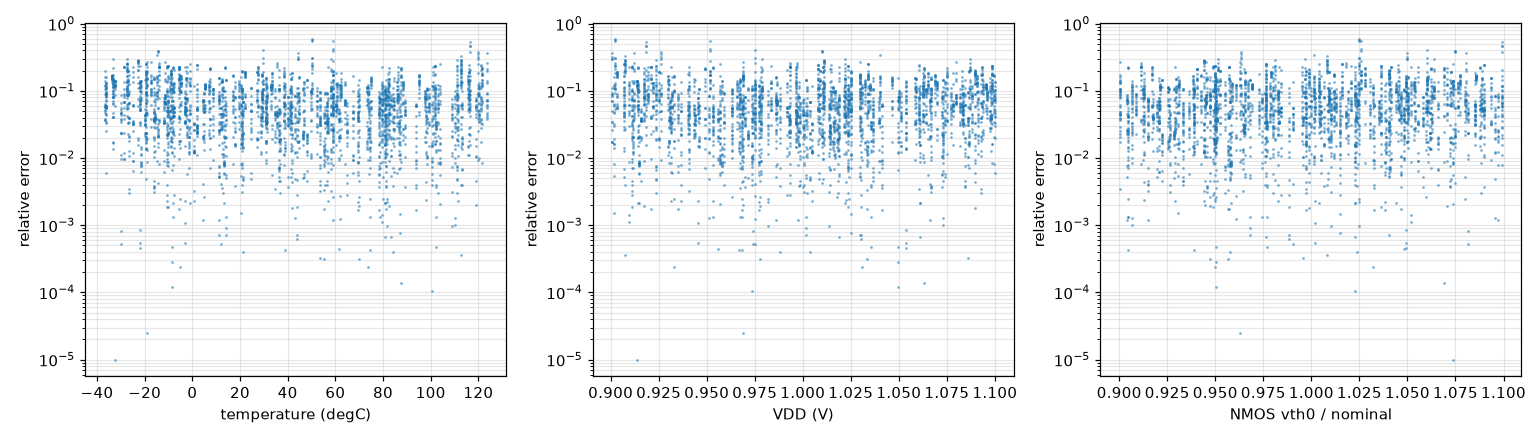
\includegraphics[width=\textwidth]{gate_error_vs_corner.png}
\caption{Gate level: relative error of all 3{,}600 runs against temperature, $\Vdd$ and the NMOS vth0 draw.}\label{fig:gcorner}
\end{figure}

\subsection{Where the largest errors occur}
\paragraph{High temperature.} The clearest dependence is on temperature (\cref{tab:gatecond}). Below $80\,^\circ$C the gate-level median error is
0.16--0.18\,\% and the P95 0.8--1.0\,\%; between $80$ and $125\,^\circ$C the median doubles to 0.33\,\%, the P95 rises to 2.2\,\%, the bias turns
negative ($-0.33$\,\%), and all of the ten largest errors occur above $100\,^\circ$C (\cref{tab:worst}).

\paragraph{Supply voltage.} The two ends of the $\Vdd$ range are slightly worse than the middle (P95 1.9\,\% and 1.3\,\% against 0.9--1.0\,\%), as
expected at the border of the sampled input range, where the networks have fewer neighbouring training points.

\paragraph{Process.} There is no systematic dependence on the vth0 draw: the median error is 0.16--0.20\,\% in every quarter of the NMOS and PMOS
vth0 range. A low threshold therefore matters only through the higher OFF current it causes (next paragraph), not by itself.
\begin{table}[H]
\centering
{\small
\begin{adjustbox}{max width=\linewidth}
\begin{tabular}{llrrrrr}
\toprule
condition & range & runs & bias & median err & P95 err & max err \\
\midrule
temperature [C] & -40 to 0 & 954 & 0.22\% & 0.16\% & 0.84\% & 2.89\% \\
temperature [C] & 0 to 40 & 846 & 0.16\% & 0.18\% & 0.76\% & 2.02\% \\
temperature [C] & 40 to 80 & 900 & 0.06\% & 0.17\% & 1.01\% & 3.26\% \\
temperature [C] & 80 to 125 & 900 & -0.33\% & 0.33\% & 2.24\% & 5.68\% \\
VDD [V] & 0.9 to 0.95 & 774 & -0.06\% & 0.25\% & 1.86\% & 5.68\% \\
VDD [V] & 0.95 to 1 & 936 & 0.06\% & 0.17\% & 0.98\% & 3.00\% \\
VDD [V] & 1 to 1.05 & 972 & 0.07\% & 0.16\% & 0.91\% & 4.66\% \\
VDD [V] & 1.05 to 1.1 & 918 & 0.03\% & 0.21\% & 1.25\% & 5.54\% \\
NMOS vth0 deviation & -10\% to -5\% & 936 & -0.01\% & 0.19\% & 1.25\% & 5.54\% \\
NMOS vth0 deviation & -5\% to +0\% & 918 & -0.01\% & 0.20\% & 1.50\% & 5.68\% \\
NMOS vth0 deviation & +0\% to +5\% & 1008 & 0.06\% & 0.17\% & 0.99\% & 5.07\% \\
NMOS vth0 deviation & +5\% to +10\% & 738 & 0.08\% & 0.20\% & 1.16\% & 3.26\% \\
PMOS vth0 deviation & -10\% to -5\% & 954 & -0.08\% & 0.20\% & 1.66\% & 4.75\% \\
PMOS vth0 deviation & -5\% to +0\% & 774 & 0.03\% & 0.16\% & 1.08\% & 5.07\% \\
PMOS vth0 deviation & +0\% to +5\% & 990 & 0.12\% & 0.20\% & 1.05\% & 5.54\% \\
PMOS vth0 deviation & +5\% to +10\% & 882 & 0.03\% & 0.20\% & 0.96\% & 5.68\% \\
\bottomrule
\end{tabular}
\end{adjustbox}
}
\caption{Gate-level (3{,}600 runs) error grouped by corner condition (vth0 deviation relative to the nominal value; negative = lower $|V_{th}|$).}
\label{tab:gatecond}
\end{table}


\begin{table}[H]
\centering
{\small
\begin{adjustbox}{max width=\linewidth}
\begin{tabular}{lrrrrrrrr}
\toprule
case & corner & VDD [V] & T [C] & NMOS vth0 [V] & PMOS vth0 [V] & SPICE [A] & ML [A] & error \\
\midrule
INV 0 & 45 & 0.9263 & 119.7 & 0.6634 & -0.6834 & $1.30\times10^{-11}$ & $1.22\times10^{-11}$ & -5.68\% \\
INV 0 & 168 & 1.073 & 110.1 & 0.6243 & -0.6481 & $7.16\times10^{-11}$ & $6.76\times10^{-11}$ & -5.54\% \\
INV 0 & 115 & 0.9074 & 112.8 & 0.6943 & -0.6089 & $9.08\times10^{-12}$ & $8.62\times10^{-12}$ & -5.07\% \\
NOR2 10 & 30 & 1.098 & 121.7 & 0.7078 & -0.6213 & $4.69\times10^{-11}$ & $4.92\times10^{-11}$ & 4.94\% \\
INV 0 & 54 & 1.098 & 101.6 & 0.6539 & -0.5767 & $3.40\times10^{-11}$ & $3.24\times10^{-11}$ & -4.75\% \\
NOR2 10 & 193 & 1.015 & 116.2 & 0.7198 & -0.5786 & $4.63\times10^{-11}$ & $4.41\times10^{-11}$ & -4.66\% \\
OR2 01 & 54 & 1.098 & 101.6 & 0.6539 & -0.5767 & $2.51\times10^{-10}$ & $2.40\times10^{-10}$ & -4.60\% \\
INV 0 & 83 & 1.062 & 120.2 & 0.6737 & -0.6936 & $2.20\times10^{-11}$ & $2.10\times10^{-11}$ & -4.59\% \\
NOR2 01 & 54 & 1.098 & 101.6 & 0.6539 & -0.5767 & $2.17\times10^{-10}$ & $2.07\times10^{-10}$ & -4.58\% \\
NOR2 00 & 45 & 0.9263 & 119.7 & 0.6634 & -0.6834 & $3.33\times10^{-11}$ & $3.18\times10^{-11}$ & -4.42\% \\
\bottomrule
\end{tabular}
\end{adjustbox}
}
\caption{The ten gate runs with the largest error and their corner conditions.}
\label{tab:worst}
\end{table}



\paragraph{Gates and input combinations.} INV\,0 accounts for five of the ten worst runs, followed by NOR2\,10 and the gates that contain an
inverter or a NOR2 stage with the same transistor states (OR2\,01, NOR2\,01, NOR2\,00).

\subsection{Why: the share of sub-threshold leakage}
For this low-power card the gate leakage at room temperature is almost entirely gate-oxide tunnelling of the ON transistors, which the ON models predict
to 0.1--0.6\,\%. Tunnelling depends only weakly on temperature, whereas the sub-threshold current of the OFF transistors grows by a factor of about
400 from $-40$ to $125\,^\circ$C (\cref{fig:trends}). \Cref{tab:offshare} quantifies this for the inverter, where exactly one transistor is OFF: the
OFF channel current carries 0.2\,\% (INV\,0) and 1.3\,\% (INV\,1) of the leakage below $0\,^\circ$C, but 13\,\% and 30\,\% above $80\,^\circ$C.
At hot corners the leakage is therefore increasingly set by the OFF channel-current models, whose errors (median 1--3\,\%, \cref{tab:chosen,tab:rails})
are an order of magnitude larger than those of the ON gate-current models. The error of the gate grows accordingly, from 0.09\,\% to 0.93\,\% median
for INV\,0. In addition, $125\,^\circ$C is the upper edge of the sampled temperature range, where the networks extrapolate least well, which explains
the small negative bias there. The same mechanism explains the least accurate gate cases (\cref{sec:gates}): INV\,0, INV\,1 and NOR2\,10 have a single
OFF device (the NOR2\,10 one is the wide $4\Lmin$ upper PMOS) carrying a large share of the leakage, whereas in NAND2\,00/10 the leakage is dominated
by ON-PMOS tunnelling and the error is 0.1\,\%.
\begin{table}[H]
\centering
{\small
\begin{adjustbox}{max width=\linewidth}
\begin{tabular}{llrrrr}
\toprule
case & T [C] & runs & OFF-channel share of leakage & median err & bias \\
\midrule
INV 0 & -40 to 0 & 53 & 0.16\% & 0.09\% & 0.04\% \\
INV 0 & 0 to 40 & 47 & 0.99\% & 0.13\% & -0.15\% \\
INV 0 & 40 to 80 & 50 & 4.56\% & 0.20\% & -0.41\% \\
INV 0 & 80 to 125 & 50 & 13.01\% & 0.93\% & -1.42\% \\
INV 1 & -40 to 0 & 53 & 1.26\% & 0.31\% & 0.45\% \\
INV 1 & 0 to 40 & 47 & 3.33\% & 0.34\% & 0.20\% \\
INV 1 & 40 to 80 & 50 & 14.47\% & 0.24\% & 0.03\% \\
INV 1 & 80 to 125 & 50 & 30.17\% & 0.66\% & -0.66\% \\
\bottomrule
\end{tabular}
\end{adjustbox}
}
\caption{Inverter: share of the leakage carried by the channel (sub-threshold) current of the OFF transistor, and the ML error, by temperature.}
\label{tab:offshare}
\end{table}



\subsection{Circuit level: corner-systematic error}
\begin{figure}[!htbp]\centering
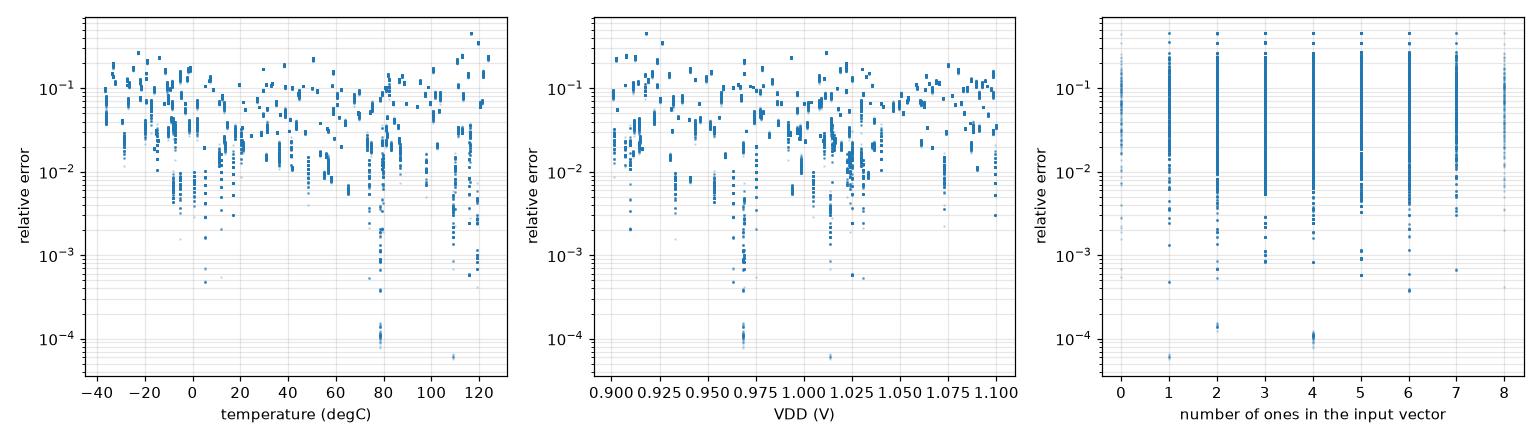
\includegraphics[width=\textwidth]{circuit_error_vs_corner.png}
\caption{Parity checker: relative error of all 51{,}200 runs against temperature, $\Vdd$ and the number of ones in the input vector.}\label{fig:ccorner}
\end{figure}
The circuit errors form vertical stripes in \cref{fig:ccorner}: at a given corner all 256 input vectors have almost the same error. The standard
deviation of the error between input vectors at one corner is only 0.011\,\%, while the mean error of a corner varies by 0.33\,\% (standard
deviation) between corners. All 28 gates of one evaluation share $\Vdd$, temperature and the process draw, so they share the systematic part of the
model error, which therefore does not average out over the circuit; only the random part does. The circuit inherits the temperature and $\Vdd$
dependence of the gates in weakened form (\cref{tab:circuitcond}): the median error is 0.25\,\% between $80$ and $125\,^\circ$C against 0.17--0.19\,\%
below, and the largest circuit error (1.6\,\%) occurs at the low end of the $\Vdd$ range.
\begin{table}[H]
\centering
{\small
\begin{adjustbox}{max width=\linewidth}
\begin{tabular}{llrrrrr}
\toprule
condition & range & runs & bias & median err & P95 err & max err \\
\midrule
temperature [C] & -40 to 0 & 13568 & 0.17\% & 0.19\% & 0.61\% & 0.80\% \\
temperature [C] & 0 to 40 & 12032 & 0.22\% & 0.18\% & 0.79\% & 0.85\% \\
temperature [C] & 40 to 80 & 12800 & 0.17\% & 0.17\% & 0.87\% & 1.63\% \\
temperature [C] & 80 to 125 & 12800 & -0.01\% & 0.25\% & 0.88\% & 1.35\% \\
VDD [V] & 0.9 to 0.95 & 11008 & 0.09\% & 0.23\% & 0.91\% & 1.63\% \\
VDD [V] & 0.95 to 1 & 13312 & 0.16\% & 0.18\% & 0.64\% & 1.05\% \\
VDD [V] & 1 to 1.05 & 13824 & 0.16\% & 0.18\% & 0.75\% & 1.01\% \\
VDD [V] & 1.05 to 1.1 & 13056 & 0.13\% & 0.25\% & 0.82\% & 0.88\% \\
NMOS vth0 deviation & -10\% to -5\% & 13312 & 0.14\% & 0.18\% & 0.74\% & 0.83\% \\
NMOS vth0 deviation & -5\% to +0\% & 13056 & 0.09\% & 0.17\% & 0.79\% & 1.07\% \\
NMOS vth0 deviation & +0\% to +5\% & 14336 & 0.17\% & 0.20\% & 0.75\% & 1.01\% \\
NMOS vth0 deviation & +5\% to +10\% & 10496 & 0.16\% & 0.28\% & 1.04\% & 1.63\% \\
PMOS vth0 deviation & -10\% to -5\% & 13568 & -0.02\% & 0.19\% & 0.87\% & 1.63\% \\
PMOS vth0 deviation & -5\% to +0\% & 11008 & 0.11\% & 0.13\% & 0.58\% & 0.79\% \\
PMOS vth0 deviation & +0\% to +5\% & 14080 & 0.28\% & 0.25\% & 0.86\% & 1.05\% \\
PMOS vth0 deviation & +5\% to +10\% & 12544 & 0.19\% & 0.21\% & 0.63\% & 0.82\% \\
\bottomrule
\end{tabular}
\end{adjustbox}
}
\caption{Parity-checker (51{,}200 runs) error grouped by corner condition (vth0 deviation relative to the nominal value; negative = lower $|V_{th}|$).}
\label{tab:circuitcond}
\end{table}



\subsection{Transistor level}
At transistor level the largest relative errors occur for the ON-state drain and source currents at small $V_{ds}$, where the channel current
passes through zero and changes sign (\cref{tab:chosen}). These currents do not enter the leakage (\cref{sec:gates_method}). The gate current of the
OFF devices lies entirely below the $10^{-15}$\,A numerical floor of the reference and cannot be learned or scored; its contribution to the leakage is
correspondingly negligible.

\subsection{Reference quality}
With the mandated tolerances alone, 3.5\,\% of the gate SPICE runs were invalid or did not converge (\cref{tab:ref}). Without the cross-check, these
runs would have appeared as ML errors of up to 100\,\%, although they are errors of the reference.
